\documentclass[a4paper]{article}

%use the english line for english reports
%usepackage[english]{babel}
\usepackage[portuguese]{babel}
\usepackage[utf8]{inputenc}
\usepackage{indentfirst}
\usepackage{graphicx}
\usepackage{verbatim}


\begin{document}

\setlength{\textwidth}{16cm}
\setlength{\textheight}{22cm}

\title{\Huge\textbf{Breakthru}\linebreak\linebreak\linebreak
\Large\textbf{Relatório Intercalar}\linebreak\linebreak
\linebreak\linebreak

\includegraphics[scale=0.1]{feup-logo.png}\linebreak\linebreak
\linebreak\linebreak
\Large{Mestrado Integrado em Engenharia Informática e Computação} \linebreak\linebreak
\Large{Programação em Lógica}\linebreak
}

\author{\textbf{Grupo Breakthru 2:}\\
João Rafael de Figueiredo Cabral - 201304395 \\
João Bernardo Martins de Sousa e Silva Mota - 201303462 \\
\linebreak\linebreak \\
 \\ Faculdade de Engenharia da Universidade do Porto \\ Rua Roberto Frias, s\/n, 4200-465 Porto, Portugal \linebreak\linebreak\linebreak
\linebreak\linebreak\vspace{1cm}}

\maketitle
\thispagestyle{empty}

%************************************************************************************************
%************************************************************************************************

\newpage

%Todas as figuras devem ser referidas no texto. %\ref{fig:codigoFigura}
%
%%Exemplo de código para inserção de figuras
%%\begin{figure}[h!]
%%\begin{center}
%%escolher entre uma das seguintes três linhas:
%%\includegraphics[height=20cm,width=15cm]{path relativo da imagem}
%%\includegraphics[scale=0.5]{path relativo da imagem}
%%\includegraphics{path relativo da imagem}
%%\caption{legenda da figura}
%%\label{fig:codigoFigura}
%%\end{center}
%%\end{figure}
%
%
%\textit{Para escrever em itálico}
%\textbf{Para escrever em negrito}
%Para escrever em letra normal
%``Para escrever texto entre aspas''
%
%Para fazer parágrafo, deixar uma linha em branco.
%
%Como fazer bullet points:
%\begin{itemize}
	%\item Item1
	%\item Item2
%\end{itemize}
%
%Como enumerar itens:
%\begin{enumerate}
	%\item Item 1
	%\item Item 2
%\end{enumerate}
%
%\begin{quote}``Isto é uma citação''\end{quote}


%%%%%%%%%%%%%%%%%%%%%%%%%%
\section{O Jogo Breakthru}
O \emph{Breakthru} é um jogo de estratégia abstrata para dois jogadores em que cada lado começa com um número diferente de peças, colocadas em posições assimétricas e com objetivos diferentes para assegurar a vitória.

\subsection{História}
O jogo foi criado em 1965 por Alex Randolph, com um conjunto de regras baseados nas do \emph{Hnefatafl}\footnote{https://boardgamegeek.com/boardgame/335/breakthru}, um jogo de estratégia abstrata cuja popularidade remonta à Escandinávia medieval, existindo vestigios da sua presença entre várias civilizações antigas\footnote{https://boardgamegeek.com/boardgame/2932/hnefatafl}.
\

\subsection{Regras}
\subsubsection{Peças}
A cor de cada jogador é sorteada através do lançamento de uma moeda, sendo que o jogador vencedor desse sorteio é o jogador dourado e o perdedor é o jogador prateado. O tabuleiro conta com 13 peças douradas, das quais 12 dispostas em quadrado à volta da 13ª peça, no centro do tabuleiro, e de 20 peças prateadas dispostas em volta das peças douradas.

O jogador dourado dispõe as suas 12 peças normais como desejar na zona central do tabuleiro, nele delimitada. O jogador prateado procede de forma semelhante, dispondo contudo as suas 20 peças fora da zona central, reservada ao jogador dourado.

Uma das peças douradas é diferente das restantes, sendo designada por navio almirante. A sua posição inicial é fixa, sendo obrigatório que seja colocada no centro do tabuleiro.

\subsubsection{Movimentos e Capturas}
Cada jogador deve, na sua vez, efetuar dois movimentos ou uma captura. 

Todas as peças podem ser movimentadas um número arbitrário de espaços livres na horizontal ou vertical, a semelhança do movimento de uma torre no xadrez. Durante o movimento nenhuma peça pode saltar por cima de outra ou ocupar uma casa já ocupada, como ilustrado na figura \ref{fig:moves}.

As capturas são feitas movimentando uma peça para uma casas que lhe seja diagonalmente adjacente e que esteja ocupada por uma peça do adversário, como ilustrado na figura \ref{fig:captures}, sendo esta removida do jogo.

Quando o navio almirante dourado efetua um movimento o jogador dourado não pode efetuar outro movimento nesse turno.

\subsubsection{Objetivo do Jogo}
O jogador prateado ganha o jogo ao capturar o navio almirante dourado. O jogador dourado ganha o jogo se o navio almirante chegar a uma das casas exteriores do tabuleiro.

\begin{figure}
\centering
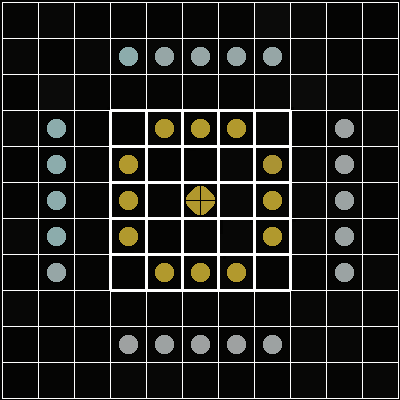
\includegraphics[scale=1]{Breakthru_board.png} 
\centering 
\caption{Uma posição inicial possível das peças num tabuleiro de Breakthru}
\label{fig:init}
\end{figure}
\begin{figure}
\centering
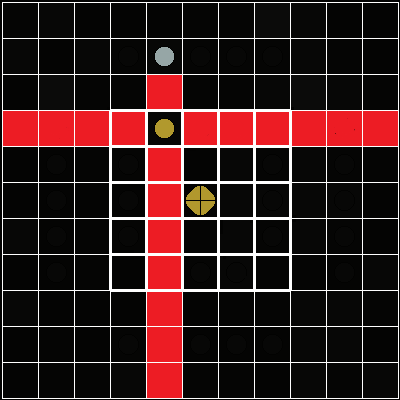
\includegraphics[scale=1]{Breakthru_moves.png}
\caption{A vermelho: movimentos possíveis da peça dourada}
\label{fig:captures}
\end{figure}

\begin{figure}
\centering
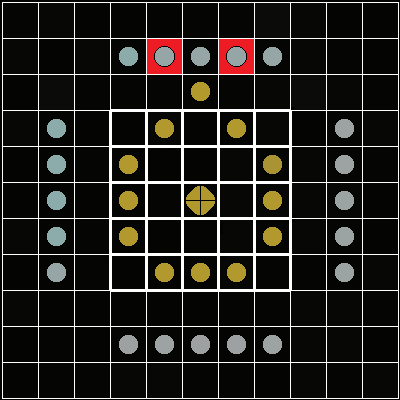
\includegraphics[scale=1]{Breakthru_capture.png}
\caption{A vermelho: capturas possíveis da peça dourada}
\label{fig:moves}
\end{figure}



%%%%%%%%%%%%%%%%%%%%%%%%%%
\section{Representação do Estado do Jogo}
O tabuleiro é representado como uma lista de listas. De seguida apresentam-se  exemplos de tabuleiros iniciais, intermédios e finais criados em Prolog.

Possível estado inicial:

\begin{verbatim} 
[[' ',' ',' ',' ',' ',' ',' ',' ',' ',' ',' '],
 [' ',' ',' ','p','p','p','p','p',' ',' ',' '],
 [' ',' ',' ',' ',' ',' ',' ',' ',' ',' ',' '],
 [' ','p',' ',' ','d','d','d',' ',' ','p',' '],
 [' ','p',' ','d',' ',' ',' ','d',' ','p',' '],
 [' ','p',' ','d',' ','F',' ','d',' ','p',' '],
 [' ','p',' ','d',' ',' ',' ','d',' ','p',' '],
 [' ','p',' ',' ','d','d','d',' ',' ','p',' '],
 [' ',' ',' ',' ',' ',' ',' ',' ',' ',' ',' '],
 [' ',' ','p','p','p','p','p','p',' ',' ',' '],
 [' ',' ',' ',' ',' ',' ',' ',' ',' ',' ',' '] ] 
\end{verbatim}

Possível estado intermédio:
\begin{verbatim}
[[' ',' ',' ',' ',' ',' ',' ',' ',' ',' ',' '],
 [' ',' ',' ','p','p',' ','d','p',' ',' ',' '],
 [' ',' ',' ','d',' ',' ',' ',' ',' ',' ',' '],
 [' ',' ',' ','p','d',' ','d','p',' ',' ',' '],
 [' ','p',' ',' ',' ','p',' ','d',' ','p',' '],
 [' ','p',' ','d',' ','F',' ','d',' ','p',' '],
 [' ','p',' ','d',' ',' ',' ','d',' ','p',' '],
 [' ','p',' ',' ','d','d','d',' ',' ','p',' '],
 [' ',' ',' ',' ',' ',' ',' ',' ',' ',' ',' '],
 [' ',' ','p','p','p','p','p','p',' ',' ',' '],
 [' ',' ',' ',' ',' ',' ',' ',' ',' ',' ',' '] ]
\end{verbatim}

Possível estado final, onde as peças douradas venceram porque o navio almirante atingiu uma das casas exteriores:
\begin{verbatim}
[[' ',' ',' ',' ',' ',' ',' ',' ',' ',' ',' '],
 [' ',' ',' ','p','p',' ','d','p',' ',' ',' '],
 [' ',' ',' ','d',' ',' ',' ',' ',' ',' ',' '],
 [' ',' ',' ','p','d',' ','d','p',' ',' ',' '],
 [' ','p',' ',' ',' ','p',' ','d',' ','p',' '],
 [' ','p',' ','d',' ',' ',' ',' ','d','p',' '],
 [' ','p',' ','d',' ',' ',' ','d',' ','p',' '],
 [' ','p',' ','p','d',' ','d',' ',' ','p',' '],
 [' ',' ',' ',' ',' ',' ',' ',' ',' ',' ',' '],
 [' ',' ','p','','d',' ','p','p',' ',' ',' '],
 [' ',' ',' ',' ',' ','F',' ',' ',' ',' ',' '] ] 
\end{verbatim}


%%%%%%%%%%%%%%%%%%%%%%%%%%
\section{Visualização do Tabuleiro}

Foram desenvolvidos alguns predicados em Prolog para permitir a visualização do tabuleiro usando caracteres \textit{ASCII}, como exemplificado pela figura \ref{fig:example}.
\begin{figure}
\centering
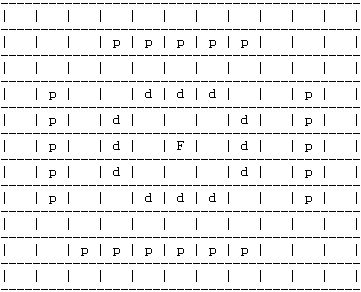
\includegraphics[scale=1]{Breakthru_initial_sicstus.png}
\caption{Tabuleiro inicial de um jogo de Breakthru}
\label{fig:example}
\end{figure}

\subsection{Predicados de Visualização}
Foram implementados os predicados de visualização que se seguem:

\begin{verbatim}
printBoard([]):-write('----------------------------------------------').
printBoard([H|T]):-
  write('---------------------------------------------'),nl,
  printLine(H, '|'), nl,
  printBoard(T).

printLine([], Sep):-
  write(Sep).
printLine([H|T], Sep):-
  write(Sep),write(' '), write(H), write(' '),
  printLine(T, Sep).
\end{verbatim}

%%%%%%%%%%%%%%%%%%%%%%%%%%
\section{Movimentos}
São possíveis movimentos simples ou capturas, para os quais se desenvolverão os predicados cujos cabeçalhos se elencam na secção \ref{sec:predicates}, que devem suceder somente se o movimento for legal ou for possível efetuar a captura, respetivamente.

\subsection{Cabeçalhos dos Predicados} \label{sec:predicates}
\begin{verbatim}
movePiece(RowOrigin, ColumnOrigin, RowDestiny, ColumnDestiny,
 Player, Board, NewBoard):-

capturePiece(RowOrigin, ColumnOrigin, RowDestiny, ColumnDestiny,
 Player, Board, NewBoard):-
\end{verbatim}


\end{document}
